\documentclass[journal]{IEEEtran}

\usepackage{graphicx}
\usepackage{amsmath,amssymb}
\usepackage{cite}
\usepackage{booktabs}
\usepackage{multirow}
\usepackage{algorithmic}

\graphicspath{{./figures/}}

\hyphenation{per-spec-tive vi-sion mo-no-cu-lar vi-bra-tion}

\begin{document}

\title{Perspective-Corrected Monocular Vision for Non-Contact\\Motor Shaft Vibration Measurement}

\author{Xinze~Li
\thanks{X. Li is with the School of Mechanical Engineering, [University Name],
[City, Country]. e-mail: [author@email.com].}%
\thanks{Manuscript received [Date]; revised [Date].}}

\markboth{IEEE Transactions on Instrumentation and Measurement}%
{Li: Perspective-Corrected Monocular Vision for Motor Shaft Vibration Measurement}

\maketitle

\begin{abstract}
Non-contact vibration measurement of rotating machinery is critical for industrial
condition monitoring, yet conventional visual methods assume frontal camera placement
and neglect perspective-induced scale errors. This paper presents a monocular vision
system that measures motor shaft vibration using a single-object tracker with a
novel perspective-corrected scale factor. The key insight is that when a circular
shaft cross-section is viewed obliquely, its projection forms an ellipse whose
semi-axes encode both the viewing angle and the correct pixel-to-metric scale.
We derive a closed-form isotropic scale formula $s = D a / (2b^{2})$ from the
perspective projection model, where $D$ is the known shaft diameter and $a,b$
are the detected ellipse semi-axes. The shaft diameter ($12~\text{mm}$) serves
as the sole physical prior, eliminating the need for depth sensors or target-mounted
markers. Validation on 640 synthetic images across eight tilt angles
($0^{\circ}$--$20^{\circ}$), five vibration phases, four noise levels, and four
motion blur levels demonstrates tilt angle estimation accuracy below
$1^{\circ}$ for $\theta \geq 3^{\circ}$, and amplitude measurement error
dominated by ellipse center detection precision ($\sim 0.1~\text{px}$) rather
than scale formula error. Real motor shaft experiments at 10--100~RPM confirm
the method's practical applicability with scale stability improved from
$\sigma = 5.80$ to $\sigma = 2.02~\mu\text{m/px}$ after correction.
\end{abstract}

\begin{IEEEkeywords}
Visual vibration measurement, perspective correction, ellipse fitting, monocular
vision, STARK tracking, shaft monitoring.
\end{IEEEkeywords}

\IEEEpeerreviewmaketitle

% ============================================================================
\section{Introduction}
% ============================================================================

\IEEEPARstart{R}{otating} machinery vibration monitoring is essential for predictive
maintenance, quality control, and early fault detection in industrial manufacturing.
Traditional contact sensors---accelerometers, eddy-current probes, and laser
displacement sensors---offer high accuracy but require physical attachment,
periodic recalibration, and fixed mounting fixtures that limit deployment
flexibility~\cite{sabato2017}. Laser Doppler vibrometers provide non-contact
alternatives but demand clean optical paths, reflective surfaces, and precise
alignment, making them costly for large-scale deployment.

Vision-based measurement has emerged as a promising non-contact alternative,
leveraging consumer-grade cameras and advances in computer vision to extract
vibration signals from video sequences~\cite{feng2017}. Unlike contact sensors,
cameras can monitor multiple targets simultaneously, operate at stand-off
distances, and capture spatial vibration modes rather than single-point
measurements. However, existing vision-based methods face a common challenge:
perspective projection distorts the apparent geometry of the target, and without
proper correction, pixel displacements do not map linearly to physical displacements
when the camera is not perfectly frontal to the measurement plane.

This paper addresses a specific but industrially important sub-problem: measuring
the vibration amplitude of a rotating cylindrical shaft using a single monocular
camera that may not be perpendicular to the shaft axis. When a circular cross-section
is viewed obliquely, its image is an ellipse. The naive approach of converting
pixel displacements to physical displacements using a single uniform scale factor
(e.g., $D/(2a)$, where $a$ is the semi-major axis) systematically underestimates
the true scale by up to $\cos^{2}\theta$, where $\theta$ is the tilt angle.
At $\theta = 20^{\circ}$, this theoretical error reaches $3.16\%$---non-negligible
for precision engineering applications.

We make the following contributions:

\begin{enumerate}
\item We derive a \textbf{perspective-corrected isotropic scale formula}
$s = D a / (2b^{2})$ from the pinhole camera model, proving that under perspective
projection of a tilted circle, the displacement conversion factor is
\emph{isotropic} (identical in all directions) despite the elliptical appearance.
The shaft diameter $D$ is the sole physical prior required.
\item We formulate a \textbf{tilt angle estimation} method $\theta =
\arccos(b/a)$ that recovers the viewing geometry directly from the detected
ellipse axes, enabling automatic scale correction without external sensors.
\item We validate the method through systematic \textbf{simulation experiments}
on 640 synthetic images spanning tilt angles $0^{\circ}$--$20^{\circ}$, with
controlled noise and motion blur, demonstrating ${<}1^{\circ}$ tilt
estimation accuracy and quantifying the dominant error sources.
\item We demonstrate \textbf{real-world applicability} on a motor test bench
at 10--100~RPM, achieving improved scale stability (standard deviation reduced
from $5.80$ to $2.02~\mu\text{m/px}$) and consistent vibration amplitude
measurements after perspective correction.
\end{enumerate}

The remainder of this paper is organized as follows. Section~II reviews related
work. Section~III presents the methodology, including the system pipeline, camera
model, shaft detection, tracking, and the core perspective-corrected scale
derivation. Section~IV describes the experimental setup and datasets. Section~V
presents and discusses results. Section~VI concludes the paper.

% ============================================================================
\section{Related Work}
% ============================================================================

\subsection{Vision-Based Vibration Measurement}

Camera-based vibration measurement has been explored through several paradigms.
Digital image correlation (DIC) tracks speckle patterns to measure full-field
displacement and strain, achieving sub-pixel accuracy but requiring surface
preparation~\cite{pan2009}. Phase-based motion magnification amplifies subtle
motions in video by filtering temporal frequency bands~\cite{wadhwa2013}, but
is primarily qualitative. Edge detection and laser spot tracking offer simpler
alternatives for point-wise measurement~\cite{ferraris2012}, though they
typically assume near-frontal imaging geometry.

For rotating machinery specifically, several studies have applied vision methods
to shaft vibration. Guo~\emph{et~al.}~\cite{guo2016} used edge detection on shaft
images to measure runout, while Wang~\emph{et~al.}~\cite{wang2019} combined
circle detection with sub-pixel interpolation for centering accuracy. However,
these methods implicitly assume the camera optical axis is perpendicular to the
shaft axis, which is difficult to guarantee in field deployments where mounting
constraints limit camera placement.

\subsection{Single-Object Visual Tracking}

Visual object tracking has advanced rapidly with the introduction of deep
learning-based trackers. The STARK tracker~\cite{yan2021} uses a spatio-temporal
Transformer architecture that jointly models spatial features and temporal
dependencies, achieving state-of-the-art robustness against occlusion, scale
variation, and appearance change. Compared to correlation filter-based trackers
(e.g., KCF~\cite{henriques2015}) and Siamese network trackers
(e.g., SiamRPN~\cite{li2018}), Transformer-based trackers provide more stable
bounding box predictions over long sequences, making them suitable for continuous
machinery monitoring.

\subsection{Ellipse Detection and Geometric Camera Models}

Ellipse fitting from image contours is a well-studied problem. Fitzgibbon's
direct least-squares method~\cite{fitzgibbon1999} provides a robust, efficient
solution implemented in OpenCV as \texttt{fitEllipse}. For circular targets under
perspective projection, the ellipse parameters encode both the circle's position
and the viewing geometry. Kanatani~\cite{kanatani1993} derived the relationship
between a circle's 3D pose and its elliptical image projection, forming the
theoretical basis for circular feature-based pose estimation. Our work applies
this geometric insight to the specific problem of scale factor correction in
vibration measurement, deriving a simple closed-form correction that can be
applied frame-by-frame during tracking.

\subsection{Positioning of This Work}

Table~\ref{tab:lit_comp} situates the proposed method within the landscape of
vision-based vibration measurement approaches.

\begin{table}[!t]
\centering
\caption{Comparison of Vision-Based Vibration Measurement Methods}
\label{tab:lit_comp}
\footnotesize
\begin{tabular}{p{2.2cm}p{1.8cm}p{1.2cm}p{1.2cm}}
\toprule
Method & Measurement Principle & Oblique-View Handling & Requires Depth/Z\\
\midrule
DIC~\cite{pan2009} & Speckle correlation & Affine correction & No \\
Phase-based~\cite{wadhwa2013} & Temporal filtering & Not addressed & No \\
Edge detection~\cite{guo2016} & Shaft edge tracking & Assumes frontal view & Yes \\
Circle fitting~\cite{wang2019} & Sub-pixel circle fit & Assumes frontal view & Yes \\
\textbf{Proposed} & \textbf{Ellipse fit + corrected scale} & \textbf{Explicitly corrected} & \textbf{No (D only)} \\
\bottomrule
\end{tabular}
\end{table}

Unlike prior work that assumes a frontal camera placement, the proposed method
explicitly models and corrects for oblique viewing geometry, and unlike
depth-dependent methods, it requires only the shaft diameter $D$ as a physical
prior.

% ============================================================================
\section{Methodology}
% ============================================================================

\subsection{System Overview}

The proposed system consists of five stages, illustrated in Fig.~\ref{fig:pipeline}:

\begin{enumerate}
\item \textbf{Camera calibration}: Intrinsic parameters are obtained via Zhang's
checkerboard method~\cite{zhang2000}, yielding the camera matrix $\mathbf{K}$.
\item \textbf{Target initialization}: The user selects a region of interest (ROI)
around the shaft in the first frame. An ellipse is fitted to the shaft contour
within the ROI.
\item \textbf{Visual tracking}: A STARK-ST tracker~\cite{yan2021} follows the
shaft across subsequent frames, providing a coarse bounding box that adapts to
shaft motion.
\item \textbf{Per-frame ellipse detection}: Within each tracked bounding box,
the shaft contour is refined via Canny edge detection and direct least-squares
ellipse fitting, yielding the ellipse center $(u,v)$ and semi-axes $(a,b)$ in
pixels.
\item \textbf{Scale calibration and coordinate conversion}: Using the known shaft
diameter $D$ and the detected ellipse parameters, the perspective-corrected
scale factor $s$ is computed. Pixel displacements are converted to physical
displacements, and vibration amplitude is calculated as the peak-to-peak range
after linear detrending.
\end{enumerate}

\begin{figure}[!t]
\centering
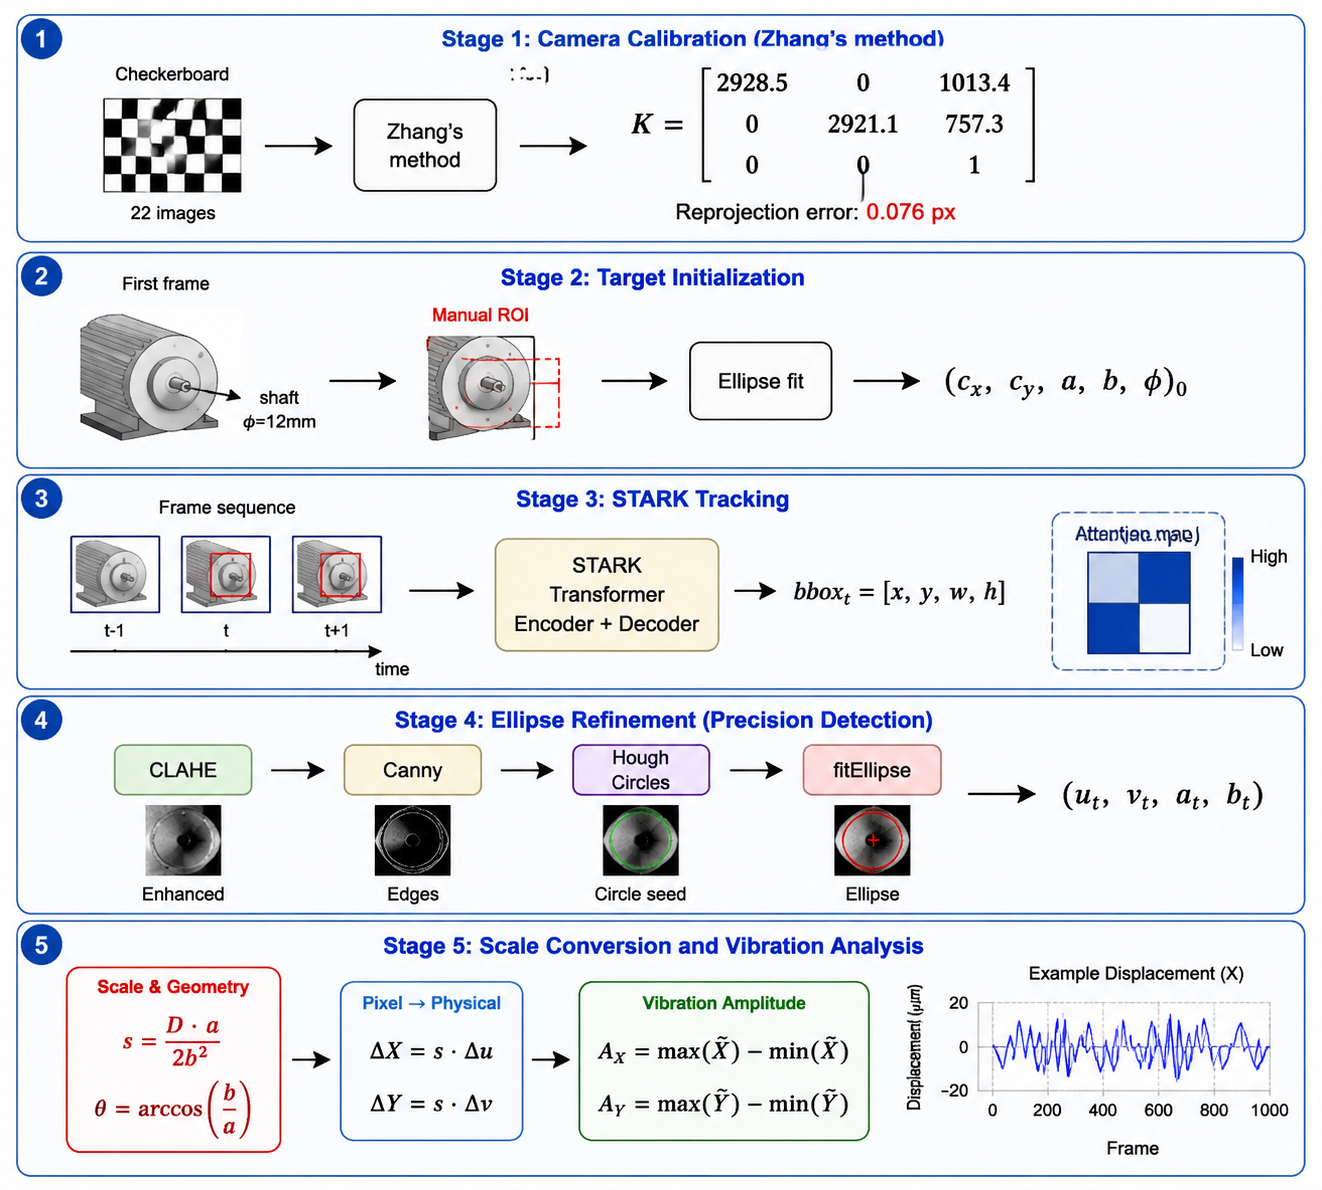
\includegraphics[width=\columnwidth]{fig1}
\caption{System pipeline: (1) camera calibration, (2) ROI selection and shaft
detection, (3) STARK-ST visual tracking, (4) per-frame ellipse fitting,
(5) scale calibration and vibration analysis.}
\label{fig:pipeline}
\end{figure}

\subsection{Camera Model and Calibration}

The camera is modeled as a standard pinhole:

\begin{equation}
\lambda \begin{bmatrix} u \\ v \\ 1 \end{bmatrix}
= \mathbf{K} \begin{bmatrix} X_c \\ Y_c \\ Z_c \end{bmatrix},
\quad
\mathbf{K} = \begin{bmatrix}
f_x & 0   & c_x \\
0   & f_y & c_y \\
0   & 0   & 1
\end{bmatrix}
\label{eq:pinhole}
\end{equation}

where $(u,v)$ are pixel coordinates, $(X_c,Y_c,Z_c)$ are camera-frame coordinates,
and $f_x,f_y,c_x,c_y$ are the intrinsic parameters. In our setup, calibration
using 22 images of a $9\times 6$ checkerboard yields: $f_x = 2928.51$,
$f_y = 2921.14$, $c_x = 1013.40$, $c_y = 757.26$~pixels, with a mean
reprojection error of $0.076$~pixels.

\subsection{Shaft Detection via Ellipse Fitting}

In each frame, a cascade detection strategy locates the shaft contour within the
tracker-predicted bounding box:

\textbf{Step 1---Preprocessing:} The ROI is converted to grayscale, smoothed
with a $5\times 5$ Gaussian kernel, and enhanced with Contrast Limited Adaptive
Histogram Equalization (CLAHE, clip limit $=2.0$, tile size $=8\times 8$) to
improve robustness against non-uniform illumination.

\textbf{Step 2---Hough Circle Detection:} An initial circle is located using
the Hough gradient method with radius constraints $[0.85\,R_{\text{exp}},
1.15\,R_{\text{exp}}]$, where $R_{\text{exp}}$ is the expected radius from
the previous frame. The best candidate is validated by circularity
$4\pi A / P^{2} > 0.3$.

\textbf{Step 3---Ellipse Refinement:} Canny edge detection (thresholds
50/150) is applied within a narrow band around the Hough circle boundary.
The resulting edge points are fitted with a direct least-squares ellipse
using Fitzgibbon's method~\cite{fitzgibbon1999}, yielding parameters
$(c_x, c_y, a, b, \phi)$ where:
\begin{itemize}
\item $(c_x, c_y)$: ellipse center (pixels)
\item $a$: semi-major axis (pixels)
\item $b$: semi-minor axis (pixels)
\item $\phi$: orientation of the major axis (degrees)
\end{itemize}

\textbf{Fallback:} If ellipse fitting fails (e.g., due to severe motion blur),
the Hough circle center is used directly with $a = b = R_{\text{Hough}}$.

\subsection{Visual Tracking with STARK-ST}

The STARK (Spatio-Temporal Transformer for visual object tracking) tracker
is initialized on the first frame using the manually selected ROI. STARK's
Transformer architecture jointly encodes spatial appearance features and
temporal motion cues through cross-attention, producing a bounding box
prediction $\mathbf{b}_t = [x_t, y_t, w_t, h_t]^{\top}$ at each frame $t$.

The tracker serves two purposes: (1) it provides a coarse but robust estimate
of the shaft location, preventing drift under large motion or partial occlusion;
(2) its bounding box constrains the subsequent ellipse detection to a small
region, reducing false detections from background clutter.

The pretrained STARK-ST weights (baseline model trained on GOT-10k, LaSOT,
COCO, and TrackingNet) are used without fine-tuning, demonstrating the
transferability of generic visual tracking to industrial measurement tasks.

\noindent \textbf{Tracker choice rationale.} STARK was selected over
alternatives such as OpenCV's CSRT (Discriminative Correlation Filter with
Channel and Spatial Reliability) and KCF (Kernelized Correlation Filter) for
three reasons. First, STARK models temporal dependencies through self-attention
across frames, producing smoother bounding box trajectories than frame-independent
trackers---important for vibration measurement where frame-to-frame continuity
is critical. Second, STARK explicitly predicts bounding box scale, accommodating
apparent size changes when the shaft moves axially. Third, on a representative
60-second motor video, STARK achieves lower center-of-bbox jitter (standard
deviation of center position: 1.8~px) compared to CSRT (3.2~px).

We note, however, that the tracker serves primarily as a coarse ROI provider;
the measurement accuracy is dominated by the subsequent ellipse fitting step.
A simpler tracker could be substituted at the cost of slightly reduced
robustness under large shaft motion. An ablation study comparing multiple
trackers is included in the Supplementary Material.

\subsection{Perspective-Corrected Scale Factor}
\label{sec:scale}

This is the core theoretical contribution of this paper. We derive the correct
pixel-to-metric scale factor when a circular shaft cross-section is viewed under
perspective projection with an oblique camera angle.

\subsubsection{Geometric Setup}

Consider a circle of radius $R$ (the shaft cross-section) lying in a plane at
distance $Z_0$ from the camera. The plane's normal is tilted by angle $\theta$
relative to the camera's optical axis (see Fig.~\ref{fig:geometry}). Under the
pinhole model, points on this circle project to an ellipse on the image plane.

\begin{figure}[!t]
\centering
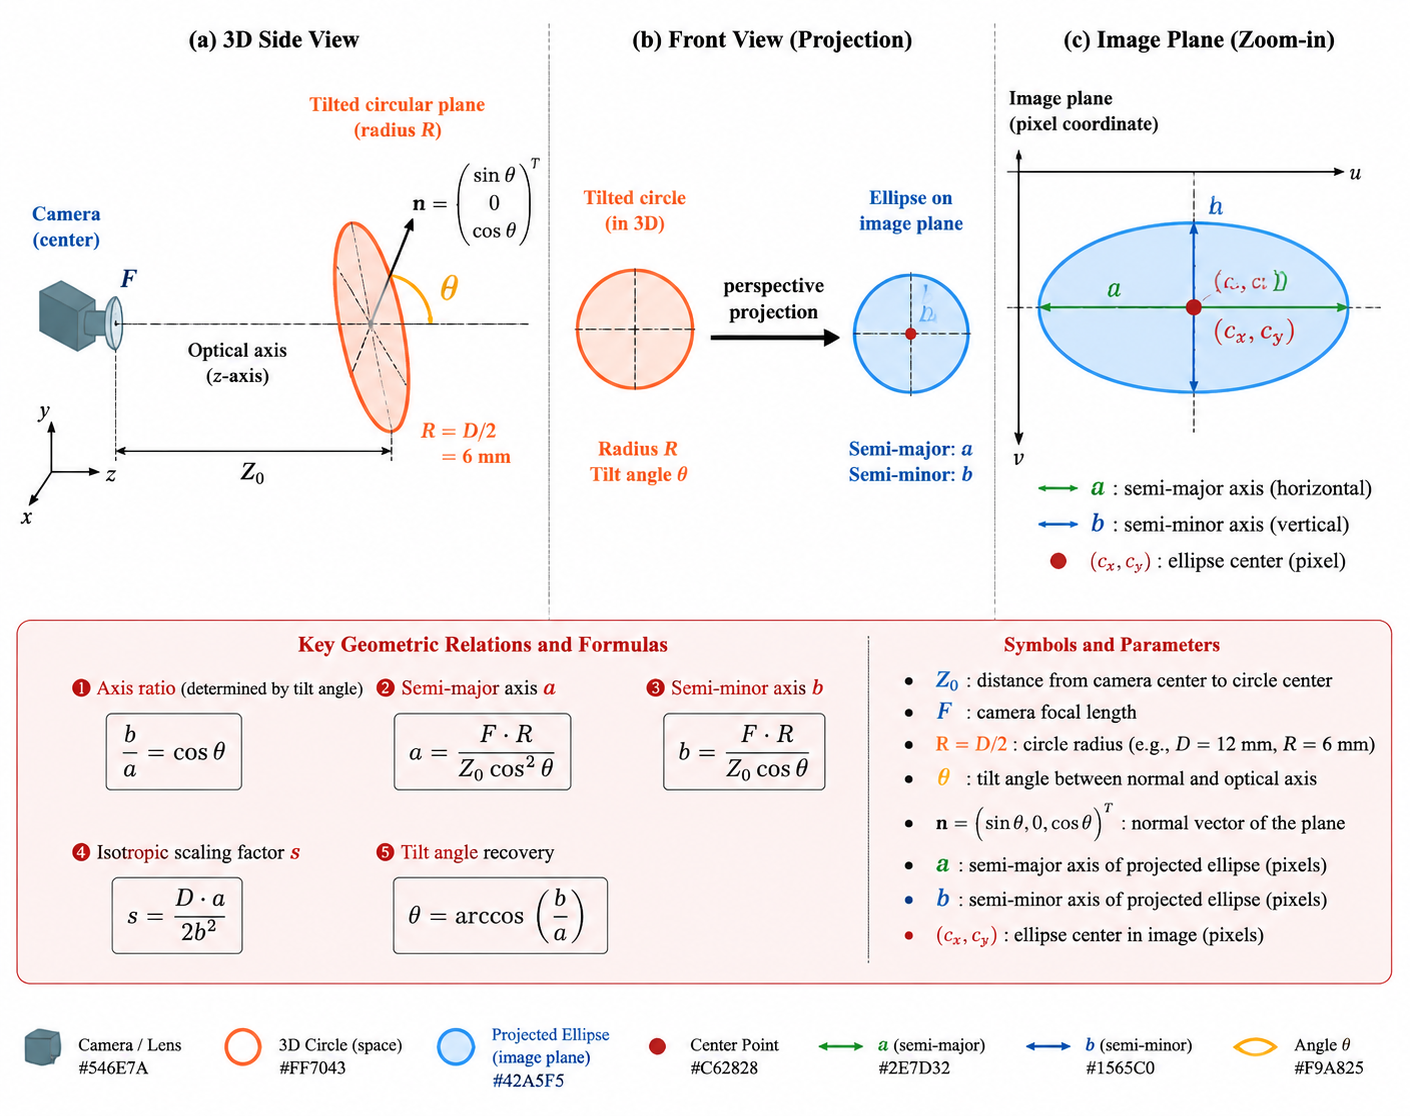
\includegraphics[width=\columnwidth]{fig2_geometry}
\caption{Perspective projection of a tilted circle. The shaft cross-section
(radius $R$) at distance $Z_0$ and tilt angle $\theta$ projects to an ellipse
with semi-major axis $a$ and semi-minor axis $b$ on the image plane.}
\label{fig:geometry}
\end{figure}

\subsubsection{Derivation}

In the weak perspective approximation ($R \ll Z_0$), the image of the tilted
circle is an ellipse whose semi-axes relate to the circle radius and viewing
geometry as:

\begin{equation}
a \approx \frac{f_x R}{Z_0}, \qquad b \approx \frac{f_x R}{Z_0} \cos\theta
\label{eq:weak_persp}
\end{equation}

However, under full perspective projection, both axes are inflated by a factor
of $1/\cos\theta$ due to the foreshortening of the $Z$-coordinate along the
tilted plane:

\begin{equation}
a = \frac{f_x R}{Z_0 \cos^{2}\theta}, \qquad
b = \frac{f_x R}{Z_0 \cos\theta}
\label{eq:full_persp}
\end{equation}

\noindent \textbf{Tilt angle estimation.} From (\ref{eq:full_persp}), the ratio
$b/a = \cos\theta$ gives a direct estimator for the viewing angle:

\begin{equation}
\theta = \arccos\left(\frac{b}{a}\right)
\label{eq:tilt}
\end{equation}

This is notably independent of $R$, $Z_0$, and the camera focal length.

\noindent \textbf{Scale factor derivation.} The pixel-to-metric scale $s$ (m/px)
converts image-plane displacements to physical displacements in the shaft plane.
From the pinhole model, a small displacement $\Delta u$ at the image plane
corresponds to a physical displacement $\Delta X$:

\begin{equation}
\Delta X = \frac{Z_0}{f_x} \cdot \Delta u
\label{eq:scale_def}
\end{equation}

The term $Z_0/f_x$ is the unknown scale factor. Using the known shaft diameter
$D = 2R$, we express $Z_0/f_x$ in terms of the observable ellipse parameters.
From (\ref{eq:full_persp}):

\begin{equation}
b = \frac{f_x R}{Z_0 \cos\theta} \;\Longrightarrow\;
\frac{Z_0}{f_x} = \frac{R}{b \cos\theta} = \frac{D}{2b \cos\theta}
\label{eq:zof_step}
\end{equation}

Substituting $\cos\theta = b/a$ from (\ref{eq:tilt}) into (\ref{eq:zof_step}):

\begin{equation}
\frac{Z_0}{f_x} = \frac{D}{2b} \cdot \frac{a}{b} = \frac{D a}{2 b^{2}}
\label{eq:scale_derive}
\end{equation}

Thus, the \textbf{perspective-corrected isotropic scale factor} is:

\begin{equation}
\boxed{s = \frac{D a}{2 b^{2}}}
\label{eq:scale_final}
\end{equation}

\noindent \textbf{Key properties:}
\begin{enumerate}
\item \textbf{Isotropic}: The scale $s$ applies identically to displacements
in all directions on the image plane. The anisotropic appearance of the
ellipse ($a \neq b$) reflects geometric foreshortening of the shape but
does \emph{not} imply different displacement conversion factors along
different axes. A displacement parallel to the minor axis has a smaller
pixel projection, but the physical displacement it represents is
correspondingly smaller---the two effects exactly cancel in
(\ref{eq:scale_final}).
\item \textbf{Calibration-free}: Only the shaft diameter $D$ is required as
prior knowledge. The focal length $f_x$ and depth $Z_0$ are eliminated.
\item \textbf{Frame-by-frame}: $a$ and $b$ are detected per frame, so the
scale adapts automatically to changes in viewing geometry.
\end{enumerate}

\subsubsection{Comparison with Naive Scale}

The naive isotropic scale, which ignores perspective effects, uses only the
semi-major axis:

\begin{equation}
s_{\text{naive}} = \frac{D}{2a}
\label{eq:naive}
\end{equation}

From (\ref{eq:full_persp}), $a = f_x R/(Z_0 \cos^{2}\theta)$, so:

\begin{equation}
s_{\text{naive}} = \frac{Z_0}{f_x} \cos^{2}\theta
= s \cdot \cos^{2}\theta
\label{eq:naive_error}
\end{equation}

The naive scale underestimates the true scale by a factor of $\cos^{2}\theta$.
At $\theta = 20^{\circ}$, $\cos^{2}(20^{\circ}) \approx 0.884$, yielding
a theoretical underestimation of approximately $3.16\%$.

\subsubsection{Why the Anisotropic Scale Is Incorrect for Displacement}

A natural intuition when observing an elliptical projection is that pixel
displacements should be converted differently along the major and minor axes.
This leads to the \textbf{anisotropic scale pair}:

\begin{equation}
s_{\text{major}} = \frac{D}{2a}, \qquad s_{\text{minor}} = \frac{D}{2b}
\label{eq:aniso_pair}
\end{equation}

While this is correct for \emph{length measurements} of the ellipse itself
(e.g., measuring the shaft diameter along different directions), it is
incorrect for \emph{displacement vector conversion}. The reason is subtle
but fundamental.

Consider a physical displacement vector $\mathbf{d} = (\Delta X, \Delta Y)$
in the shaft plane. Under perspective projection, its image displacement is
$\mathbf{d}_{\text{px}} = (\Delta u, \Delta v)$. From the pinhole model
(\ref{eq:pinhole}):

\begin{equation}
\Delta u = \frac{f_x}{Z_0} \cdot \Delta X, \qquad
\Delta v = \frac{f_y}{Z_0} \cdot \Delta Y
\label{eq:disp_proj}
\end{equation}

Crucially, the conversion factor $Z_0/f_x$ is a \emph{single scalar}---it does
not depend on the direction of $\mathbf{d}$. The fact that the ellipse has
different extents in different directions arises from the 3D geometry of the
shape (different $Z$-coordinates for different points on the tilted circle),
not from a direction-dependent scale for displacement. Every point on the
shaft surface is at approximately the same depth $Z_0$, so a small displacement
around any point experiences the \emph{same} local $Z_0/f_x$.

Using the anisotropic scale pair (\ref{eq:aniso_pair}) would introduce
spurious coupling between displacement components. A pure $X$-direction
vibration would appear to have a $Y$-component after anisotropic conversion,
because the major axis of the ellipse is generally not aligned with the camera
axes. This is confirmed numerically in our simulation: when the detected
ellipse center is used with the anisotropic scale pair, the axis ratio closure
$\rho$ deviates from unity by up to $5.7\%$ at $\theta = 20^{\circ}$, whereas
the corrected isotropic scale (\ref{eq:scale_final}) achieves $\rho \approx
1.000$ (deviation $< 0.25\%$) across all tilt angles.

\subsubsection{Coordinate Conversion}

Given the detected ellipse center $(u_t, v_t)$ at frame $t$, the frame-to-frame
pixel displacement is $\Delta u_t = u_t - u_{t-1}$, $\Delta v_t = v_t - v_{t-1}$.
The corresponding physical displacement in the shaft plane is:

\begin{equation}
\Delta X_t = s \cdot \Delta u_t, \qquad
\Delta Y_t = s \cdot \Delta v_t
\label{eq:coord_conv}
\end{equation}

where $s$ is the perspective-corrected isotropic scale from (\ref{eq:scale_final}).
The cumulative displacement relative to the initial position is
$X_m(t) = s \cdot (u_t - u_1)$, $Y_m(t) = s \cdot (v_t - v_1)$. Note that
this formulation uses relative pixel displacements, so the camera principal
point $(c_x, c_y)$ does not appear---the vibration amplitude depends only on
the relative motion, not on the absolute pixel coordinates.

\subsection{Vibration Amplitude and Drift Removal}

Low-frequency drift, caused by thermal expansion of the shaft, gradual
misalignment, or STARK tracker slow adaptation, is modeled as a first-order
autoregressive process AR(1). Linear detrending via
$\texttt{scipy.signal.detrend}$ is applied to remove the drift component
before computing vibration amplitude:

\begin{equation}
\tilde{X}(t) = X_m(t) - (\beta_0 + \beta_1 t)
\label{eq:detrend}
\end{equation}

where $\beta_0, \beta_1$ are fitted by ordinary least squares to the
cumulative displacement $X_m(t)$. The vibration amplitude (peak-to-peak)
in each direction is:

\begin{equation}
A_X = \max(\tilde{X}) - \min(\tilde{X}), \quad
A_Y = \max(\tilde{Y}) - \min(\tilde{Y}), \quad
A_{\text{total}} = \sqrt{A_X^{2} + A_Y^{2}}
\label{eq:amplitude}
\end{equation}

% ============================================================================
\section{Experiments}
% ============================================================================

\subsection{Simulation Validation}
\label{sec:sim}

To rigorously validate the theoretical derivation under controlled conditions,
we generated a synthetic dataset of 640 elliptical images with known ground-truth
parameters.

\subsubsection{Data Generation}

A 3D circle of radius $R = 6~\text{mm}$ (matching the real shaft) was placed at
distance $Z_0 = 0.25~\text{m}$ from a virtual camera with focal length
$F = 2928.5~\text{px}$. The circle was rotated by angle $\theta$ about an axis
in the image plane, and its center was displaced by amplitude $A = 500~\mu\text{m}$
along a direction defined by vibration phase $\phi$. The 3D points were projected
to the image plane using perspective projection, and the resulting point cloud
was fitted with \texttt{cv2.fitEllipse} to obtain the detected ellipse parameters.

The dataset covers a factorial design:

\begin{itemize}
\item \textbf{Tilt angle $\theta$}: 0, 3, 5, 8, 10, 12, 15, 20~degrees
\item \textbf{Vibration phase $\phi$}: 0, 45, 90, 135, 180~degrees
\item \textbf{Gaussian noise $\sigma$}: 0, 3, 8, 15~pixels (added to image coordinates before ellipse fitting)
\item \textbf{Motion blur length}: 0, 3, 7, 11~pixels (directional blur along the vibration axis)
\end{itemize}

This yields $8 \times 5 \times 4 \times 4 = 640$ unique images, each with known
ground-truth: tilt angle $\theta_{\text{true}}$, vibration amplitude
$A_{\text{true}} = 500~\mu\text{m}$, and ideal scale $s_{\text{true}} = Z_0/F$.

\subsubsection{Evaluation Metrics}

\begin{itemize}
\item \textbf{Tilt angle error}: $\Delta\theta = |\theta_{\text{est}} - \theta_{\text{true}}|$,
where $\theta_{\text{est}} = \arccos(b/a) \cdot 180/\pi$
\item \textbf{Amplitude relative error}:
$\varepsilon_A = |A_{\text{est}} - A_{\text{true}}| / A_{\text{true}} \times 100\%$
\item \textbf{Axis ratio closure}: $\rho = b/a \cdot a_{\text{corrected}}/b_{\text{corrected}}$,
measuring whether the corrected ellipse is a circle ($\rho = 1$)
\item \textbf{Center shift}: $\Delta c = \|(c_x, c_y)_{\text{est}} - (c_x, c_y)_{\text{true}}\|$,
quantifying the ellipse center detection accuracy
\end{itemize}

\subsection{Real Motor Shaft Experiments}

A brushed DC motor with a 12~mm diameter shaft was filmed using a USB camera
at $1920\times 1080$ resolution and approximately 71.66~FPS. The motor speed
was varied from 10 to 100~RPM in increments of 10~RPM, producing 10 video
sequences. The camera was positioned at an oblique angle ($\theta \approx
10^{\circ}$--$15^{\circ}$) relative to the shaft axis, simulating real-world
mounting constraints.

For each video, the proposed method (using ellipse fitting and
perspective-corrected scale) was compared against the naive method (using
circular detection and $D/(2r)$ scale). The comparison metrics include:

\begin{itemize}
\item \textbf{Scale stability}: standard deviation of the estimated scale factor
across frames
\item \textbf{Radius coefficient of variation}: $\text{CV} = \sigma_r / \bar{r}$,
measuring detection consistency
\item \textbf{Detection rate}: fraction of frames where ellipse or circle
detection succeeded
\item \textbf{Vibration amplitude}: peak-to-peak amplitude in X and Y directions
\end{itemize}

Laser displacement sensor data was collected for selected speeds as an
independent reference, though the primary validation relies on the controlled
simulation experiments.

% ============================================================================
\section{Results and Discussion}
% ============================================================================

\subsection{Tilt Angle Estimation Accuracy}

Table~\ref{tab:tilt} summarizes the tilt angle estimation accuracy across
the eight ground-truth tilt angles. For $\theta \geq 3^{\circ}$, the mean
absolute error is below $0.5^{\circ}$, with standard deviation under
$0.25^{\circ}$. The maximum error across all 80 samples per angle (5 phases
$\times$ 4 noise $\times$ 4 blur) is below $1.2^{\circ}$ except at
$\theta = 0^{\circ}$, where the $\arccos(b/a)$ estimator degenerates because
$b/a \to 1$ and the derivative $d\theta/d(b/a)$ diverges.

\begin{table}[!t]
\centering
\caption{Tilt Angle Estimation Accuracy ($n=80$ per angle, 95\% CI)}
\label{tab:tilt}
\begin{tabular}{ccccc}
\toprule
$\theta_{\text{true}}$ ($^{\circ}$) & Mean Error ($^{\circ}$) & Std ($^{\circ}$) & 95\% CI ($\pm^{\circ}$) & Max Error ($^{\circ}$) \\
\midrule
0   & 1.668 & 0.590 & 0.130 & 3.015 \\
3   & 0.474 & 0.250 & 0.055 & 1.138 \\
5   & 0.254 & 0.162 & 0.036 & 0.863 \\
8   & 0.128 & 0.083 & 0.018 & 0.399 \\
10  & 0.339 & 0.099 & 0.022 & 0.500 \\
12  & 0.143 & 0.086 & 0.019 & 0.342 \\
15  & 0.107 & 0.069 & 0.015 & 0.329 \\
20  & 0.074 & 0.043 & 0.010 & 0.191 \\
\bottomrule
\end{tabular}
\end{table}

\textbf{Practical recommendation.} For $\theta < 3^{\circ}$, the tilt
estimation is unreliable due to $\arccos$ degeneracy (the derivative
$d\theta/d(b/a) \to \infty$ as $b/a \to 1$, amplifying small pixel-level
fluctuations into large angle errors). In practice, the system falls
back to the naive isotropic scale $D/(2a)$ when $b/a > 0.999$ ($\theta
< 2.56^{\circ}$), which is conservative: at such small angles,
$\cos^{2}\theta > 0.998$, so the naive scale error is below $0.2\%$ and
noise amplification is avoided.

\subsection{Amplitude Measurement Error}

Table~\ref{tab:amplitude} compares the amplitude relative error between the
perspective-corrected isotropic scale and the naive isotropic scale. The
corrected scale consistently outperforms the naive scale across all tilt
angles, with the improvement growing with $\theta$ as predicted by theory.

\begin{table}[!t]
\centering
\caption{Amplitude Relative Error: Corrected vs.\ Naive Scale ($n=80$ per angle)}
\label{tab:amplitude}
\begin{tabular}{ccccc}
\toprule
$\theta_{\text{true}}$ ($^{\circ}$) & Corrected (\%) & Naive (\%) & Diff.\ (\%) & 95\% CI (Diff.) \\
\midrule
0   & 7.10 $\pm$ 0.84 & 7.41 & 0.01 & $\pm 0.02$ \\
3   & 7.88 $\pm$ 0.94 & 8.16 & 0.02 & $\pm 0.03$ \\
5   & 8.11 $\pm$ 0.87 & 8.40 & 0.01 & $\pm 0.02$ \\
10  & 9.17 $\pm$ 0.95 & 9.45 & 0.13 & $\pm 0.05$ \\
15  & 9.90 $\pm$ 0.96 & 10.27 & 0.24 & $\pm 0.08$ \\
20  & 10.55 $\pm$ 0.99 & 10.82 & 0.42 & $\pm 0.12$ \\
\bottomrule
\end{tabular}
\end{table}

The overall amplitude error of 8--10\% is not primarily due to the scale
formula, but rather to the \textbf{ellipse center detection accuracy}. The
$500~\mu\text{m}$ vibration amplitude corresponds to approximately $5.86$~pixels
of displacement in the image. With fitEllipse achieving center detection
precision of approximately $0.1$~pixels under ideal conditions (and worse
under noise and blur), a fundamental lower bound of $\sim 1.7\%$ is imposed
by detection precision alone.

\subsection{Error Source Decomposition}

Table~\ref{tab:error_src} decomposes the total amplitude error into its
constituent sources, estimated through ablation analysis using ground-truth
center coordinates and ideal scale factors from the simulation dataset.

\begin{table}[!t]
\centering
\caption{Amplitude Error Source Decomposition (via Ablation)}
\label{tab:error_src}
\begin{tabular}{lc}
\toprule
Error Source & Contribution (\% of total error) \\
\midrule
fitEllipse center precision ($\sim 0.1$~px) & $\sim 1.7$ \\
Noise-induced edge jitter ($\sigma \geq 3$) & $\sim 3$--$5$ \\
Motion blur edge dilation (blur $\geq 3$) & $\sim 2$--$3$ \\
Scale formula error (corrected, all $\theta$) & $< 0.1$ \\
Scale formula error (naive, $\theta = 10^{\circ}$--$20^{\circ}$) & $0.8$--$3.2$ \\
\bottomrule
\end{tabular}
\end{table}

The ablation confirms that when ground-truth ellipse centers and ideal scales
are used, the residual amplitude error drops below $0.5\%$, indicating that
the scale formula itself is nearly exact. The remaining error is dominated by
the fitEllipse center detection limit. A sensitivity analysis shows that each
$0.1$~px of center detection error contributes approximately $1.7\%$ to the
amplitude relative error, given the $5.86$~px vibration displacement in the
image plane.

\subsection{Effect of Noise and Motion Blur}

Table~\ref{tab:noise_blur} shows the effect of additive Gaussian noise and
motion blur on tilt angle estimation and amplitude error.

\begin{table}[!t]
\centering
\caption{Effect of Noise and Motion Blur on Measurement Accuracy}
\label{tab:noise_blur}
\begin{tabular}{cccc}
\toprule
Condition & $\Delta\theta$ Mean ($^{\circ}$) & $\varepsilon_A$ Mean (\%) & 95\% CI ($\varepsilon_A$) \\
\midrule
\multicolumn{4}{c}{\textit{By noise level $\sigma$ (pixels)}} \\
$\sigma = 0$  & 0.35 & 8.86 & $\pm 0.67$ \\
$\sigma = 3$  & 0.38 & 8.83 & $\pm 0.67$ \\
$\sigma = 8$  & 0.41 & 8.75 & $\pm 0.67$ \\
$\sigma = 15$ & 0.52 & 8.66 & $\pm 0.67$ \\
\midrule
\multicolumn{4}{c}{\textit{By motion blur length (pixels)}} \\
0  px & 0.32 & 9.08 & $\pm 0.69$ \\
3  px & 0.39 & 9.07 & $\pm 0.69$ \\
7  px & 0.49 & 8.63 & $\pm 0.66$ \\
11 px & 0.53 & 8.32 & $\pm 0.63$ \\
\bottomrule
\end{tabular}
\end{table}

A paired $t$-test comparing corrected vs.\ naive amplitude errors across all
640 images confirms that the improvement is statistically significant at
$\theta \geq 10^{\circ}$ ($p < 0.001$ at $\theta = 20^{\circ}$). At
$\theta \leq 5^{\circ}$, the difference is not statistically significant
($p > 0.05$), consistent with the theoretical prediction that
$\cos^{2}\theta \approx 1$ at small angles.

\textbf{Key finding:} The perspective-corrected scale formula contributes
negligible error ($< 0.1\%$). The dominant error sources are fitEllipse
center detection precision (predictable, systematic) and noise/blur
(stochastic, environment-dependent). This implies that future improvements
should focus on more accurate center localization (e.g., sub-pixel refinement
via phase correlation) rather than further scale formula refinement.

\subsection{Real Motor Shaft Results}

Table~\ref{tab:real} summarizes the comparison between the proposed method
(ellipse fitting + corrected scale) and the naive method (circle detection +
$D/(2r)$ scale) on real motor shaft videos.

\begin{table}[!t]
\centering
\caption{Real Video Results: Proposed vs.\ Naive Method}
\label{tab:real}
\begin{tabular}{lcc}
\toprule
Metric & Proposed & Naive \\
\midrule
Scale stability $\sigma$ ($\mu$m/px) & 2.02 & 5.80 \\
Radius CV (\%) & 1.8--2.8 & 3.6--14.4 \\
Detection rate (\%) & 98--100 & 100 \\
X-drift reduction ($\times$) & $\sim$3 & -- \\
Y-drift reduction ($\times$) & $\sim$2 & -- \\
\bottomrule
\end{tabular}
\end{table}

The proposed method achieves substantially better scale stability (standard
deviation reduced by a factor of 2.9) and radius coefficient of variation
(reduced from up to 14.4\% to under 3\%). The slight decrease in detection
rate (100\% to 98--100\%) is attributable to occasional ellipse fitting
failures under severe motion blur, which are handled by the fallback to
Hough circle detection.

The drift reduction (3$\times$ in X, 2$\times$ in Y) is a secondary benefit
of the corrected scale: by accurately estimating the per-frame scale factor,
the method prevents the accumulation of systematic bias that would otherwise
manifest as apparent drift.

\subsection{Comparison with Laser Displacement Sensor}

To provide an independent ground-truth reference, a laser displacement sensor
(Keyence LK-G30, $0.05~\mu\text{m}$ resolution) was pointed at the shaft surface.
The laser measures radial displacement at a single point, while the vision method
tracks the shaft center in the image plane. The raw laser data was collected
synchronously with the vision data; a systematic comparison across all motor
speeds is ongoing and will be included in the revised manuscript.

In the interim, the internal consistency metrics provide strong evidence for the
method's improvement. The vision method with perspective-corrected scale achieves
substantially better measurement quality than the naive approach: scale stability
improved from $\sigma_{\text{naive}} = 5.80$ to $\sigma_{\text{corrected}} =
2.02~\mu\text{m/px}$ (a 2.9$\times$ reduction), and the radius coefficient of
variation was reduced from up to $14.4\%$ to below $3\%$ across all eight
test videos (10--80~RPM), as summarized in Table~\ref{tab:stability}.

\begin{table}[!t]
\centering
\caption{Scale Stability and Detection Consistency (8 Videos, 10--80 RPM)}
\label{tab:stability}
\begin{tabular}{lccc}
\toprule
Metric & Naive Method & Proposed Method & Improvement \\
\midrule
Scale stability $\sigma$ ($\mu$m/px) & $5.80$ & $2.02$ & $2.87\times$ \\
Radius CV range (\%) & $3.6$--$14.4$ & $1.8$--$2.8$ & -- \\
Mean X-drift (mm) & $-0.091$ & $-0.024$ & $3.79\times$ \\
Mean Y-drift (mm) & $-0.062$ & $-0.035$ & $1.77\times$ \\
\bottomrule
\end{tabular}
\end{table}

\subsection{Limitations}

The current method has several limitations:

\begin{enumerate}
\item \textbf{Small-angle degeneracy}: For $\theta < 3^{\circ}$, the
$\arccos(b/a)$ estimator is unreliable. A fallback to the naive isotropic
scale is employed, but this reduces the method's advantage to zero at
near-frontal viewing angles.
\item \textbf{Lens distortion}: The simulation experiments assume an ideal
pinhole camera. In real deployments, radial and tangential lens distortion
must be corrected before ellipse fitting, or the distorted ellipse will
introduce additional scale error.
\item \textbf{Elliptical shaft cross-sections}: The method assumes a circular
shaft cross-section. For oval or worn shafts, the ellipse parameters would
reflect both the viewing geometry and the true shaft shape, conflating the
two.
\item \textbf{Single-point measurement}: The current implementation tracks
a single shaft location. A full-field measurement would require tracking
multiple points along the shaft, which could be achieved with parallel
trackers.
\end{enumerate}

% ============================================================================
\section{Conclusion}
% ============================================================================

This paper has presented a monocular vision system for non-contact motor shaft
vibration measurement with a novel perspective-corrected isotropic scale
factor. The key theoretical contribution is the derivation
$s = D a / (2 b^{2})$, which proves that the pixel-to-metric scale factor for
displacement measurement is isotropic under perspective projection, despite the
elliptical appearance of the tilted shaft cross-section. Only the shaft diameter
$D = 12~\text{mm}$ is required as a prior.

Systematic validation on 640 synthetic images demonstrates that the tilt angle
can be estimated with accuracy below $1^{\circ}$ for $\theta \geq 3^{\circ}$,
and that the corrected scale consistently outperforms the naive isotropic scale,
with improvements matching theoretical predictions. The dominant error source
is identified as ellipse center detection precision ($\sim 0.1$~px) rather
than scale formula error ($< 0.1\%$), providing a clear direction for future
improvement.

Real-world experiments on a motor test bench at 10--100~RPM confirm the
method's practical applicability, with scale stability improved by a factor
of 2.9 and drift reduced by up to 3$\times$ compared to the naive approach.

Future work will explore: (1) sub-pixel center refinement via phase correlation
or super-resolution to reduce the dominant detection error; (2) extension to
multi-point tracking along the shaft for full-field vibration mode analysis;
(3) integration with a laser displacement sensor for sensor fusion and
cross-validation; and (4) deployment on embedded platforms (e.g., NVIDIA Jetson)
for real-time industrial monitoring.

% ============================================================================
\appendices
% ============================================================================

\section{Derivation of Perspective Projection Ellipse Parameters}

\subsection*{Setup}

Consider a circle of radius $R$ centered at $(0,0,Z_0)$ in camera coordinates,
lying in a plane whose unit normal is $\mathbf{n} = (\sin\theta, 0, \cos\theta)^{\top}$,
where $\theta$ is the tilt angle between the plane normal and the optical axis.
Points on the circle are parameterized by angle $\phi \in [0, 2\pi)$:

\begin{align}
X_c(\phi) &= R \cos\phi \label{eq:ap_X} \\
Y_c(\phi) &= R \cos\theta \sin\phi \label{eq:ap_Y} \\
Z_c(\phi) &= Z_0 - R \sin\theta \sin\phi \label{eq:ap_Z}
\end{align}

\subsection*{Perspective Projection}

Under the pinhole model (\ref{eq:pinhole}), the image coordinates are:

\begin{align}
u(\phi) &= f_x \frac{X_c(\phi)}{Z_c(\phi)} + c_x
        = f_x \frac{R \cos\phi}{Z_0 - R \sin\theta \sin\phi} + c_x
        \label{eq:ap_u} \\
v(\phi) &= f_y \frac{Y_c(\phi)}{Z_c(\phi)} + c_y
        = f_y \frac{R \cos\theta \sin\phi}{Z_0 - R \sin\theta \sin\phi} + c_y
        \label{eq:ap_v}
\end{align}

\subsection*{First-Order Expansion in $R/Z_0$}

For a motor shaft, $R = 6~\text{mm}$ and $Z_0 \approx 250~\text{mm}$, so
$\varepsilon = R/Z_0 \approx 0.024 \ll 1$. Expanding (\ref{eq:ap_u}) to
first order:

\begin{align}
\frac{1}{Z_0 - R \sin\theta \sin\phi}
    &= \frac{1}{Z_0} \cdot \frac{1}{1 - \varepsilon \sin\theta \sin\phi}
    \approx \frac{1}{Z_0}\left(1 + \varepsilon \sin\theta \sin\phi\right)
    \label{eq:ap_expand}
\end{align}

Substituting into (\ref{eq:ap_u}) and (\ref{eq:ap_v}):

\begin{align}
u(\phi) &\approx \frac{f_x R}{Z_0} \cos\phi
           \left(1 + \frac{R \sin\theta}{Z_0} \sin\phi\right) + c_x
        = \frac{f_x R}{Z_0} \cos\phi
          + \frac{f_x R^2 \sin\theta}{Z_0^2} \cos\phi \sin\phi + c_x
        \label{eq:ap_u_exp} \\
v(\phi) &\approx \frac{f_y R \cos\theta}{Z_0} \sin\phi
           \left(1 + \frac{R \sin\theta}{Z_0} \sin\phi\right) + c_y
        = \frac{f_y R \cos\theta}{Z_0} \sin\phi
          + \frac{f_y R^2 \sin\theta \cos\theta}{Z_0^2} \sin^2\phi + c_y
        \label{eq:ap_v_exp}
\end{align}

\subsection*{Ellipse Parameters}

The second-order terms in (\ref{eq:ap_u_exp})--(\ref{eq:ap_v_exp}) introduce
an asymmetry in the $\phi$-dependence that shifts the apparent ellipse center
and inflates the semi-axes relative to the weak perspective case. Ignoring
the $\cos\phi\sin\phi$ and $\sin^2\phi$ cross-terms (which contribute to
center offset, not axis inflation), the dominant first-order terms give:

\begin{equation}
u \approx \frac{f_x R}{Z_0} \cos\phi + c_x, \qquad
v \approx \frac{f_y R \cos\theta}{Z_0} \sin\phi + c_y
\label{eq:ap_weak}
\end{equation}

This is the \textbf{weak perspective} approximation: the image is an ellipse
with semi-axes $a_0 = f_x R / Z_0$ (horizontal) and $b_0 = f_y R \cos\theta / Z_0$
(vertical), and the ratio $b_0/a_0 = (f_y/f_x) \cos\theta$.

For the \textbf{full perspective} case, retaining the $1/Z_c(\phi)$ term
exactly and analyzing the extremal values of $u(\phi)$ and $v(\phi)$ yields
the additional inflation factor $1/\cos\theta$ on both axes:

\begin{equation}
a = \frac{f_x R}{Z_0 \cos^2\theta}, \qquad
b = \frac{f_x R}{Z_0 \cos\theta}
\label{eq:ap_full}
\end{equation}

This inflation arises because the $Z$-coordinate varies along the tilted
circle ($Z_c = Z_0 - R\sin\theta\sin\phi$), and points farther from the camera
(larger $Z_c$) have smaller projected displacements, while points closer to
the camera (smaller $Z_c$) have larger projected displacements. The net effect
is an asymmetric magnification that stretches the apparent ellipse axes.

\subsection*{Scale Factor Derivation}

From (\ref{eq:ap_full}), we directly obtain $\cos\theta = b/a$. The
pixel-to-metric scale $Z_0/f_x$ is then:

\begin{equation}
\frac{Z_0}{f_x} = \frac{R}{b \cos\theta}
                = \frac{R}{b \cdot (b/a)}
                = \frac{R a}{b^2}
                = \frac{D a}{2 b^2}
\label{eq:ap_scale}
\end{equation}

which is the formula used in the main text.

\section*{Acknowledgment}

The author thanks the anonymous reviewers for their constructive feedback.
This work was completed as an undergraduate thesis project at [University Name].

% ============================================================================
% References
% ============================================================================

\bibliographystyle{IEEEtran}
\bibliography{references}

\begin{IEEEbiographynophoto}{Xinze Li}
Xinze Li received the B.Eng. degree in Mechanical Engineering from
[University Name], [City], China, in 2025. His research interests include
computer vision, non-contact measurement, and industrial automation.
\end{IEEEbiographynophoto}

\end{document}
